%%% -*-LaTeX-*-

\chapter{Modern NICs}
Network Interface Cards have grown complex over time and present opportunities and 
challenges as part of a modern distributed system. It is imperative that today's
database system designer treats network transmission as a first class citizen in every design decision.
Previous research for optimising databases were focussed more on processing time spent on a 
database query~\cite{dbmsproctime}, but today's truth is that lion's share of the end-to-end latency
while processing a query is spent in network transmission
Since we are not reeling from slow disks anymore, the bulk of I/O bottleneck in a distributed system today is in network transmission.
Adding this to the fact that the modern NIC allows us to offload CPU from the data transfer path,
the saved memory bandwidth and CPU cycles could be utilised for useful work 

Network cards have had TCP offloading baked in as TCP Offload Engine for some time now, but it was getting 
more and more ineffective because of performance issues and complexities involved~\cite{tcpoffload}.
RDMA~\cite{rdmapatent,rdmacase,rdma} was proving to be a much better alternative with TCP offloading where
transport offloading was just one among varios benefits involved. Development of advanced switching 
interconnects such as PCI express~\cite{pcie} made it possible to develop highly performant 
network devices offering throughputs and latencies a couple of orders of magnitudes better
than what was possble with prior transports such as TCP.


\section{Zero Copy}
Kernel bypass is a ubiquitous feature in the modern NIC and key to accessing remote memory directly 
from across the network. While the literal definition just defines any data movement that doesn't 
involve copying between user space and kernel space, even packet capturing libraries~\cite{pcap} could fall
under those definitions. Newer network controllers make use of vectored I/O, otherwise known as scatter/gather I/O
where a single procedure reads data from multiple buffers and writes it to single buffer. The Mellanox Infiniband ConnectX\textregistered-3
NIC that we profiled provides a scatter/gather list which powers it's on NIC DMA engine. This specific kernel bypass
mechanism is colloqially known as Zero Copy.

Zero copy DMA facilitates a scatter gather list of buffer descriptors
which could be mapped to non contigous locations in memory on demand. These provide
the added benefit that network headers don't need to exist along with data and helps bring more flexibility 
in deciding the transport layer. One subtle thing to note here is that Zero Copy only implies the absence 
of a memcopy from the records to a buffer. The data still needs to be copied to the on-NIC buffers before 
it is sent out via the network cable. This is different from what happens when we call socket send on a traditional 
tcp stack where the data for transmission is pre assembled in a huge buffer and then copied across the network.
We evaluate how Zero Copy performs in contrast with the more traditional network copy approach, which we will refer
to as the ``copy out" approach in later sections.

\section{Memory Bandwidth}
Interestingly, the additional copy involved in the traditional approach hurts memory bandwidth of the system more than contributing 
to additional CPU load purely from the perspective of network transmission. Our evaluation show us that while the traditional
copy just adds a modest 5\% increase in absolute CPU utilisation, making use of the high throughput available in NICs by transmitting
near line rate takes up one third of the total available memory bandwidth in a modern server. We should read this in the context that 
network transmission is not the primary responsibility of a server in a distributed system. Most of the memory bandwidth wasted in 
just aggregating the data before transmission could be used as part of actual computation or other useful rearrangement of data in 
the query response.


\section{NIC structures in detail}
\begin{figure}[t]
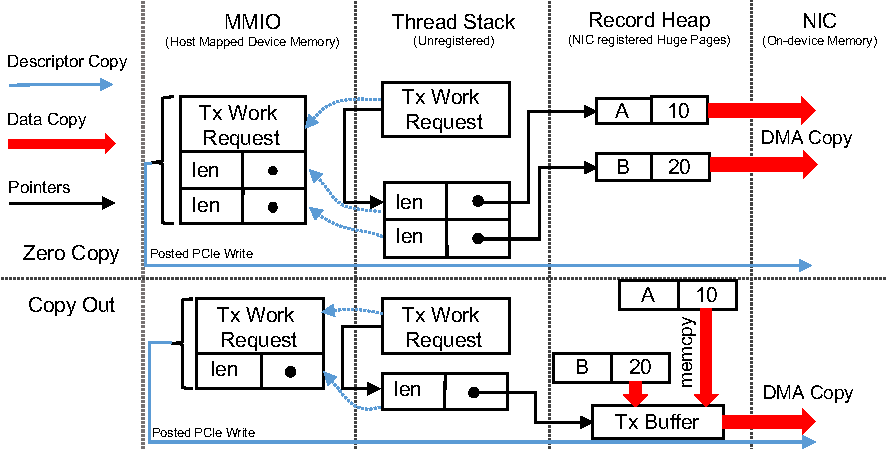
\includegraphics[width=\textwidth]{fig-mem-regions.pdf}
\caption{Key structures involved in network transmission.}
\label{fig:mem-regions}
\end{figure}

Figure~\ref{fig:mem-regions} details how an application interacts with a Mellanox
ConnectX-3\textregistered , a modern 56~Gbps NIC that uses kernel bypass. 
With zero-copy, transmit descriptors list several chunks of data for
the NIC to DMA. With copy-out, all data to be transmitted is first explicitly
copied into a transmit buffer by the host CPU; then, a transmit descriptor is
posted that references just the transmit buffer rather than the original
source data. Both zero-copy and the traditional copy-out approaches to transmission are shown.
In both cases the same three key data structures are involved. The first important structure is the
data to be transmitted, which lives in heap memory.  For zero-copy, the memory
where the records live must first be registered with the NIC. Registration
informs the NIC of the virtual-to-physical mapping of the heap pages. This is
required because the NIC must perform virtual-to-physical address translation
since the OS is not involved during transmission and the application has no
access to its own page tables.  Registration is done at startup and is often
done with physical memory backed by 1~GB hugepages to minimize on-NIC address
translation costs.

The second key structure is the descriptor that a thread must construct to
issue a transmission. With Mellanox NICs, a thread creates a work request and a
gather list on its stack. The work request indicates that the requested
operation is a transmission, and the gather list is a contiguous list of
base-bound pairs that indicate what data should be transmitted by the NIC (and
hence DMAed). For zero-copy, the gather list is as long as the number of chunks
that the host would like to transmit, up to a small limit. The NICs we use support
posting up to 32~chunks per transmit operation. Later, we find that this small
limit bottlenecks NIC transmit performance when chunks are small and numerous.

The final important structure is the control interface between the NIC and the
host CPU.  When the NIC is initially set up by the application, a region of the
NIC's memory is mapped into the application's virtual address space. The NIC
polls this region, and the host writes new descriptors to it from the thread's
stack to issue operations. The region is mapped as write-combining; filling a
cacheline in the region generates a cacheline-sized PCIe message to the NIC.
The NIC receives it, and it issues DMA operations to begin collecting the data
listed in the descriptor. The PCIe messages are posted writes, which means they
are asynchronous from the CPU's perspective. Even though PCIe latencies are much
higher than DRAM access, the CPU doesn't stall when posting descriptors, so the
exchange is very low overhead.

\subsection{Zero Copy vs Copy Out}
The key difference between zero-copy and copy-out is shown with the wide, red
arrows in Figure~\ref{fig:mem-regions}. Copy-out works much like conventional
kernel-based networking stacks: chunks of data are first copied into a single
transmit buffer in host memory. Then, a simple, single-entry descriptor is
posted to the NIC that DMAs the transmit buffer to an on-device buffer for transmission
As a result, copy-out requires an extra and explicit copy of the data, which is made
by the host CPU.  Making the copy uses host CPU cycles, consumes memory
bandwidth, and is pure overhead. Surprisingly, though, copy-out has
advantages including better performance when
records are small and scattered.  In those cases, complex gather descriptors
bottleneck the NIC, and using the host CPU to pre-assemble the responses can
improve performance.



\section{DDIO}
performance-oriented enhancements to the DMA mechanism have been introduced in 
Intel\textregistered Xeon E5 processors with their Data Direct I/O (DDIO)~\cite{ddio} feature,
allowing the DMA ``windows" to reside within CPU caches instead of system RAM. As a result,
CPU caches are used as the primary source and destination for I/O, 
allowing network interface controllers (NICs) to talk directly to the caches of local CPUs
and avoid costly fetching of the I/O data from system RAM. As a result,
DDIO reduces the overall I/O processing latency, allows processing of the I/O 
to be performed entirely in-cache, prevents the  available memory bandwidth from becoming a performance bottleneck.

We need to fully investigate the effects of DDIO in reducing memory bandwidth 
in order to conclusively comment on the impact of traditional copy mechanisms.


\section{Inlining}
Mellanox NICs allow some data to be {\em inlined} inside the control message
sent to the NIC over PCIe. Our NICs allow up to 912~B to be included inside the
descriptor that is posted to the NIC control ring buffer.  Inlining can improve
messaging latency by eliminating the delay for the NIC to DMA the message data
from host DRAM, which can only happen after the NIC receives the descriptor.
Inlining benefits small request/response exchanges, but it does not help for
larger transmissions. This is because even though there is an extra delay
before the NIC receives the actual record data, that delay can be overlapped
with the DMA and transmission of other responses. Other researchers have shown
that sending data to the NIC via MMIO also wastes PCIe bandwidth~\cite{rdma}.
Almost all of our experiments have inlining disabled. Enabling inlining
gives almost identical throughput and overhead to copy-out, except it only
works for transmissions of ~912 B or less.